\subsubsection{Experiment 1}
In Experiment 1 the performance impact of the implemented driver on \emph{Google Chrome} is measured. The internal structure of the driver was used to create the four main groups of measurement, without the driver, with the \gls{WPM} component, with the \gls{DLL} load component and with both components. This test was then done for 1, 2, 4, 8 and 16 opened tabs and data was obtained for a duration of 1, 2, 4, 8 and 16 minutes of runtime. The measurement was done with \emph{Google Chrome's} internal profiler\footnote{\url{chrome://profiler}}. In total this results in 200 data files obtained through the profiler which was then used to evaluate the performance decrease. The resulting 200 data files are merged with five different operations, minimum, maximum, median, mean and sum of all values. The titles of the resulting plots have been abbreviated to their respective function names of Section~\ref{sec:profiler}. Considering the implementation of the driver, this experiment should show that the execution without the driver is faster.
\begin{figure}[h]
	\centering
    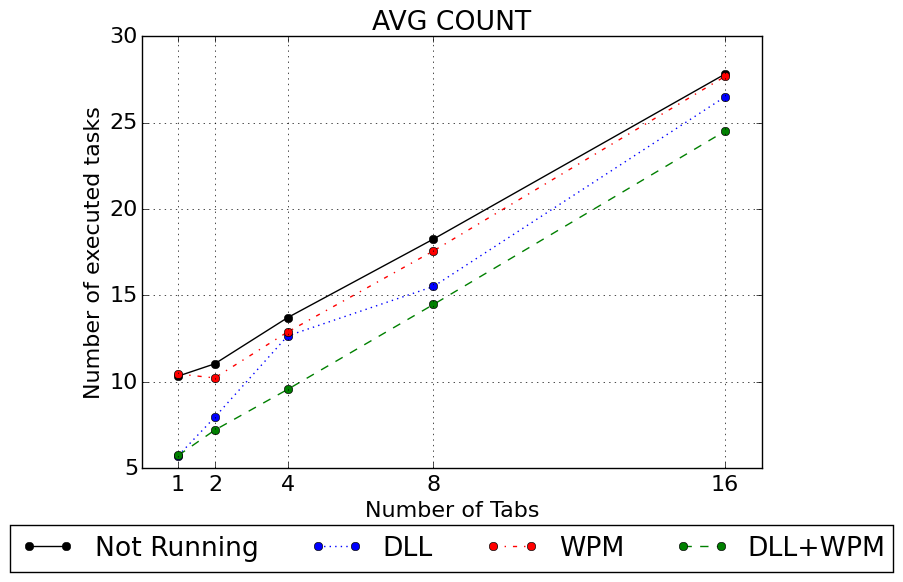
\includegraphics[width=\textwidth,height=0.45\textheight,keepaspectratio]{Evaluation/experiment1/AVG-COUNT-2.png}
    \caption{Average count, 2 minutes of data}
    \label{fig:ex1_avgcount_2}

  	\vspace*{\floatsep}
  	
    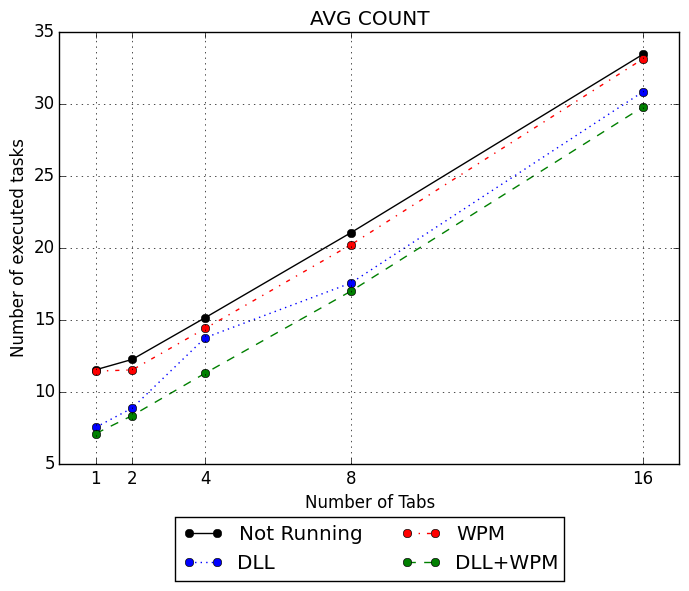
\includegraphics[width=\textwidth,height=0.45\textheight,keepaspectratio]{Evaluation/experiment1/AVG-COUNT-16.png}
    \caption{Average count, 16 minutes of data}
    \label{fig:ex1_avgcount_16}
\end{figure}
Figure~\ref{fig:ex1_avgcount_2} shows the average count of tasks that were executed over two minutes. Running both components, \emph{\gls{DLL}+\gls{WPM}} is the slowest of all four configurations, because the average number of executed tasks is the lowest. \emph{WPM} and the \emph{Not Running} are almost equal with \emph{\gls{WPM}} being one task slower in for two and fours tabs. Figure~\ref{fig:ex1_avgcount_16} shows the same measurement for a duration of 16 minutes. The result is the same as of Figure~\ref{fig:ex1_avgcount_2}. The comparison between both plots show that there is not much of a difference between a one and 16 minute measurement, but the 16 minute measurements give more accurate results. What is more interesting about these graphs is the linear trend of the four plots. For each added tab only about 1.5 times more tasks are executed. This is consistent throughout all four plots.
\begin{figure}[h]
	\centering
    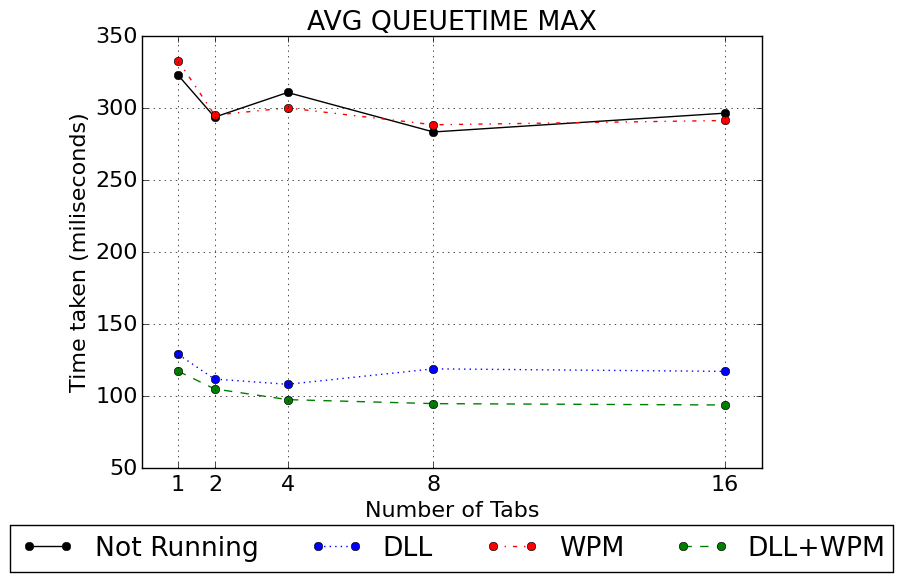
\includegraphics[width=\textwidth,height=0.45\textheight,keepaspectratio]{Evaluation/experiment1/AVG-QUEUETIME-MAX-1.png}
    \caption{Average of the maximum queuetime, 1 minute of data}
    \label{fig:ex1_avgqueuetimemax_1}

	\vspace*{\floatsep}

    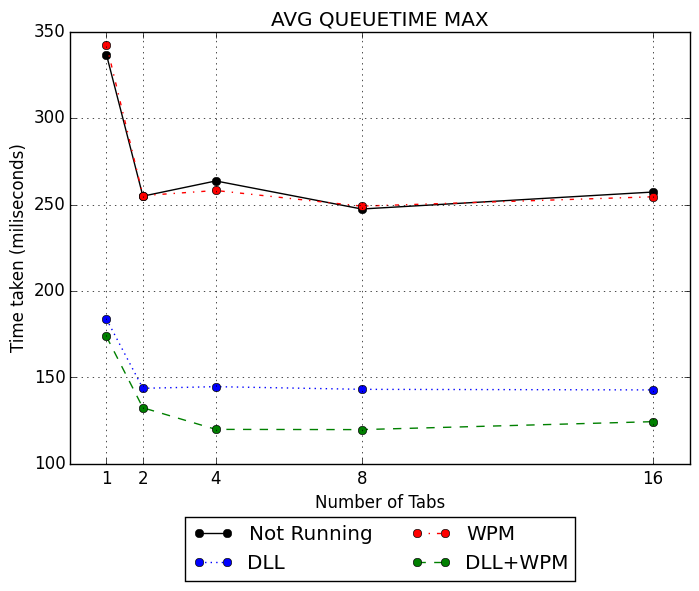
\includegraphics[width=\textwidth,height=0.45\textheight,keepaspectratio]{Evaluation/experiment1/AVG-QUEUETIME-MAX-16.png}
    \caption{Average of the maximum queuetime, 16 minutes of data}
    \label{fig:ex1_avgqueuetimemax_16}
\end{figure}
This property of \emph{Chrome} being faster (executing more task) without a driver running can be seen too in the next two Figures~\ref{fig:ex1_avgqueuetimemax_1}~and~\ref{fig:ex1_avgqueuetimemax_16}. These graphs show the average of the maximum queuetime. The y-axis shows the average number of milliseconds a task was waiting for execution. Again, two groups form, \emph{Not Running} with \emph{\gls{WPM}} and \emph{\gls{DLL}} and \emph{\gls{DLL}+\gls{WPM}}. Tasks without running driver queue in average longer than tasks with running driver. The reason for that is \emph{Not running} executes more tasks, which leads to some tasks queuing longer because Chrome is busy with running other tasks. Accordingly, the average queuetime for the \gls{DLL} component and both components running is lower, because less tasks are executed and Chrome is less busy with task execution. The overhead of the driver is clearly present in the figures and tasks are in average waiting 100 milliseconds less than without running the driver. This means, that the average overhead per task introduced to the driver is 100 milliseconds for the queuetime.
\begin{figure}[h]
	\centering
    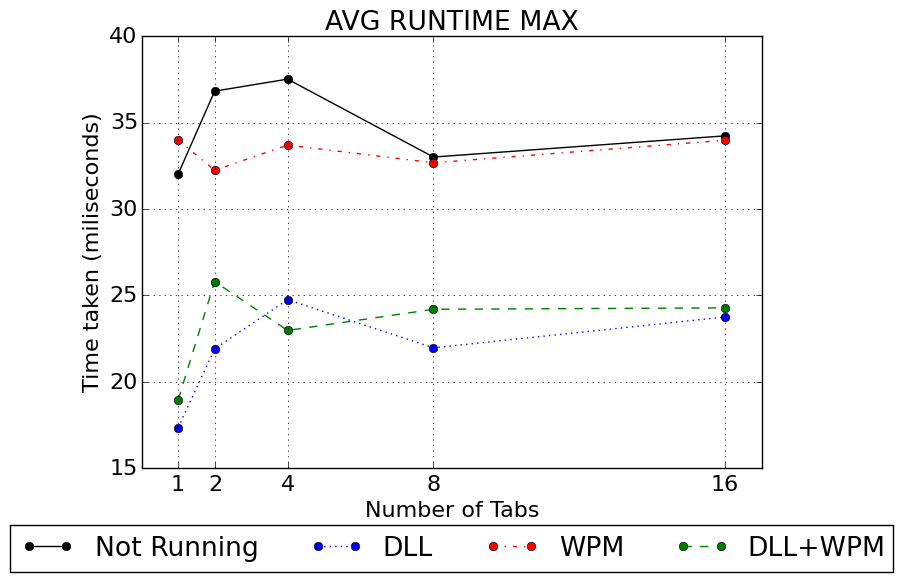
\includegraphics[width=\textwidth,height=0.45\textheight,keepaspectratio]{Evaluation/experiment1/AVG-RUNTIME-MAX-1.png}
    \caption{Average of the maximum runtime, 1 minute of data}
    \label{fig:ex1_avgruntimemax_1}
    
  	\vspace*{\floatsep}    
    
    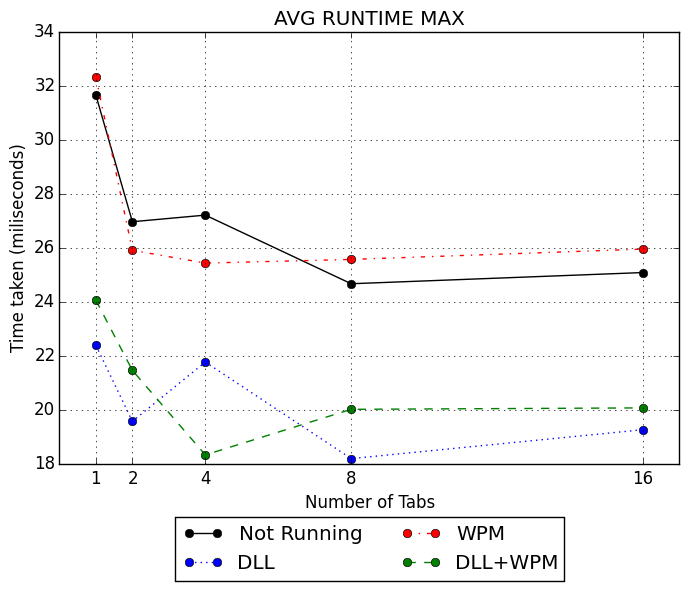
\includegraphics[width=\textwidth,height=0.45\textheight,keepaspectratio]{Evaluation/experiment1/AVG-RUNTIME-MAX-16.png}
    \caption{Average of the maximum runtime, 16 minutes of data}
    \label{fig:ex1_avgruntimemax_16}
\end{figure}
Figure~\ref{fig:ex1_avgruntimemax_1}~and~\ref{fig:ex1_avgruntimemax_16} show the average of the maximum runtime of all tasks for one and 16 minutes. The results of this plots are similar to Figure~\ref{fig:ex1_avgqueuetimemax_1}~and~ \ref{fig:ex1_avgqueuetimemax_16}. The average runtime of \emph{Not Running} and \emph{\gls{WPM}} is higher than \emph{\gls{DLL}} and \emph{\gls{DLL}+\gls{WPM}}. This is again a result of the higher number of tasks executed and \emph{Chrome} being already busy executing other tasks. Additionally, tasks are waiting for other tasks to be finished with execution, extending the runtime.
\begin{figure}[h]
	\centering
    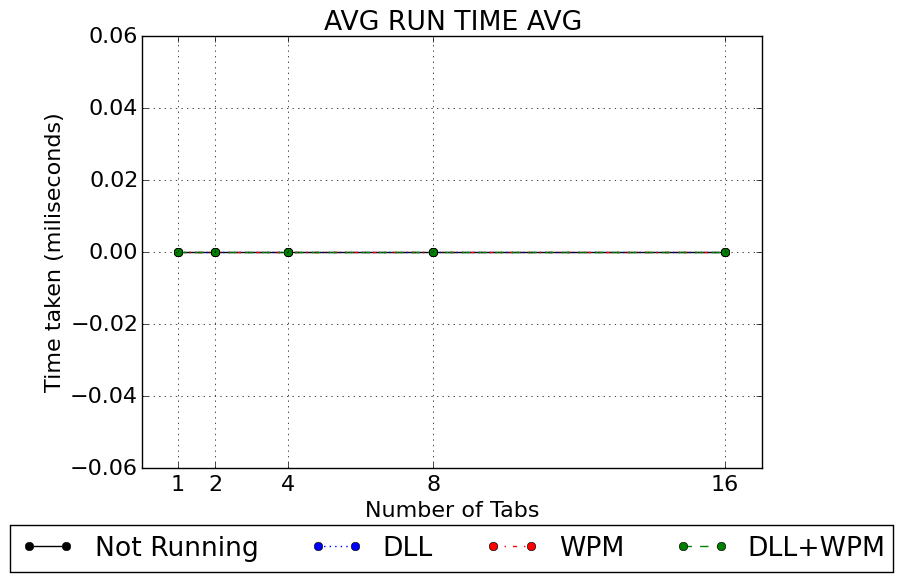
\includegraphics[width=\textwidth,height=0.45\textheight,keepaspectratio]{Evaluation/experiment1/AVG-RUNTIME-AVG-1.png}
    \caption{Average of the average runtime, 1 minute of data}
    \label{fig:ex1_avgruntimeavg_1}
    
  	\vspace*{\floatsep}    
    
    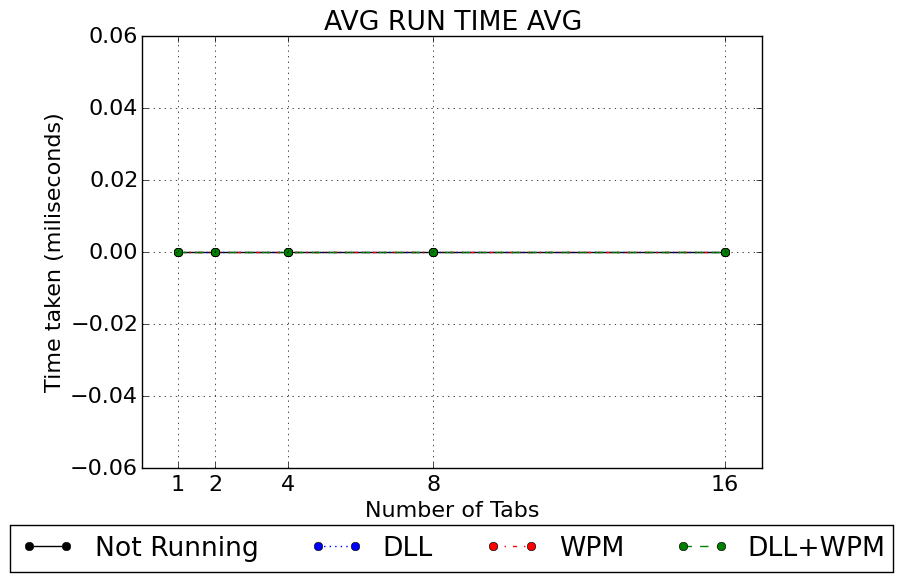
\includegraphics[width=\textwidth,height=0.45\textheight,keepaspectratio]{Evaluation/experiment1/AVG-RUNTIME-AVG-16.png}
    \caption{Average of the average runtime, 16 minutes of data}
    \label{fig:ex1_avgruntimeavg_16}
\end{figure}
At the end of this experiment, a look is taken at the average of the average runtime of a task. This data is shown in Figure~\ref{fig:ex1_avgruntimeavg_1} for one minute and Figure~\ref{fig:ex1_avgruntimeavg_16} for 16 minutes. The result is, that there is in average no difference between running the driver and not running it. For both Figures, the average runtimes are zero. This means, because the runtimes are using rounded values, the execution took less than 0.50 milliseconds in average.

\medskip

The result of this Experiment 1 is, that the driver slows down execution during startup, which increase maximum run- and queuetime. There is no difference during the later usage, as the average of the average runtimes are staying constant. The reason for this performance decrease can be found in the \gls{DLL} component of the driver, as the other one, the \gls{WPM} component is running with almost no performance decrease. The \gls{DLL} component will be evaluated further in Experiment 2.